\section{Account of the rescue}

    Will and I had planned the day before that we would go and push Cattlegrid. We woke at around 9am and took our time with waking up and preparing for the trip as it was to be a fairly short, simple trip. We had also decided to do de-rig Quantum State, the idea being that we would use the rope to drop the pitch at the end of Cattlegrid. We tried (not very hard) to convince Kenneth to join us. We were unsuccessful. DW, Tanguy and Clare also had a short trip planned, into Monatip. They were ahead of us on the entrance abseil, and we ended up on the abseil at 12pm exactly. Progress down to the end of Knot Very Good was smooth and unrushed, taking around 2 hours. We carried onto Quantum State and I de-rigged the rope, around 40(?)m of it. Before we started down Cattlegrid we stopped for some food. Will led the way down past the drips and as he had been through before, he knew how to move through the passage and so he was quicker than me. When I got to the place where I had my accident he was already past and moving just out of sight, so I hadn’t seen him go through the small hole to the left of the climb down. I noted the hole, decided it
    would be uncomfortable in comparison to the 2m free climb down. The climb wasn’t difficult; I didn’t hesitate in attempting it at least.

    I stood facing the way I had come from, found hand holds on both the left and right side. I tested them (as I had come to learn in exploration caving) and found them secure enough to trust. I don’t recall thinking of the rock that I was holding onto with my left hand as anything other than completely stable and solid. I probed downwards with my feet, and finding no decent foothold I dropped my feet slowly, taking all my weight in my arms to lower my feet down to the ground below (which must have been in reach). As I did so I watched the rock I was holding to the left move, and begin to fall. With the way it was moving the rock had no intention of supporting me. I had enough time and cognition to try and get myself out of the way, pushing off with the left hand, throwing myself face down onto the floor. The rock, or one that was dislodged along with it, struck me in the lower half of my back. 

    \begin{pagefigure}
        \checkoddpage \ifoddpage \forcerectofloat \else \forceversofloat \fi
        \centering
        \frame{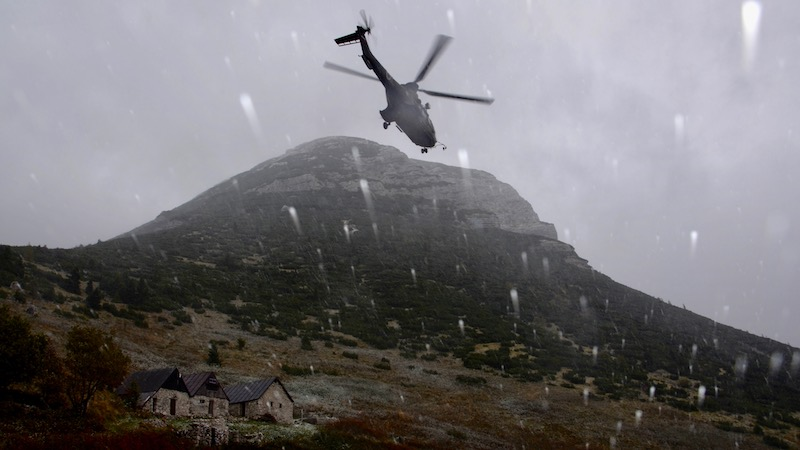
\includegraphics[width=\textwidth]{images/2016/arun-rescue-2016/dsc_0367_jani_kutin_delo_na_kalu.jpg}}
        \caption{ --- photo by Jana \v{C}arga}
        \label{helicopter}
    \end{pagefigure}

\fullwidthbox{The Slovene Cave rescue}{Because the Slovene army pilots having a flight quota to complete each year, helicopters have often heli-lifted gear and provisions to the Sheperds Hut, and even as far as the sunset spot on top of the mountain. During the rescue, however, the pilots flew directly to the cave entrance of Primadona, hovering a few metres from the cliff edge, in the black of night, playing no small part in facilitating the rescue effort. Praise must also go the 60 strong team of cavers and mountaineers drawn from across Slovenia who participated in all aspects of the rescue: from communications, cooking, blasting and bolting teams to the medics who took charge and to the JSPDT members who knew the cave and acted as guides}

    Instantly the implications of back injuries overwhelmed my thoughts. Before I even realised I was winded and in some serious pain, I tested if I was able to move my fingers and toes and limbs. Will was now at my side, having only just been far enough ahead to have not been able to see the accident. He would have heard the rocks fall, and my gasps of pain whilst I tried to get my breath back. On my hands and knees I attempted to move straight away, informing Will of what happened. That I had been hit in the back but could move despite the pain. He stopped me standing up, suggested staying where I was as I had injured by back. I decided I could and should move enough to get to the bottom of Knot Very Good, where Will said we should wait for 10/15 minutes to allow the injuries to make themselves apparent to me. We dropped all the tackle sacks and with a lot of help from Will I made it to a flat, dry rock in (what we have now named) The Waiting Room. Will went back for our equipment. We emptied the tackle sacks and I lay on them. We discussed our options at that point. It was 15:20. We were 7 hours away from our call out, 9 away from reasonably expecting to see anyone coming down for a rescue. If, after the adrenaline started to wear off I could move enough to prussick slowly, we would do that. But only if we were confident as getting stuck on the ropes halfway up a pitch would be far worse than lying down. If I couldn’t move we were to stay together and keep each other warm.

    \begin{figure}[t]
        \checkoddpage \ifoddpage \forcerectofloat \else \forceversofloat \fi
        \centering
        \frame{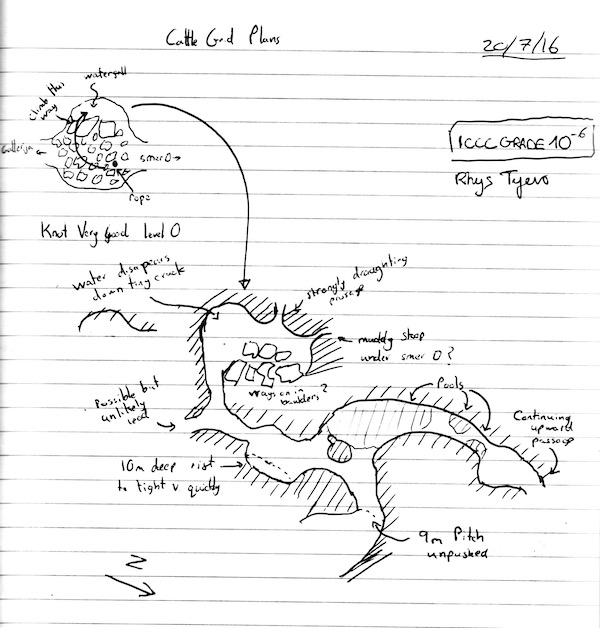
\includegraphics[width=\textwidth]{images/2016/arun-rescue-2016/migovec_cartoon_2.jpg}}
        \caption{A grade 1 survey of Cattle Grid area, including pitch to be descebded --- scanned from 2016 Bivi Logbook}
        \label{Cattlegrid}
    \end{figure}

    After about 10 minutes I got onto my hands and knees, with difficulty. With help from will I attempted to stand up. I couldn’t stretch out my legs to stand up straight. I was beginning to stiffen up. I attempted to stretch my legs when back on my hands and knees, acting out a prussicking motion. It hurt badly, I told Will that we were now just going to have to sit pretty, keep each other warm and wait for rescue. We had gotten into the plastic survival bags from our helmets, and I had taken 2 ibuprofen from the med kit. We lay down and began to wait.

    Facing a 9 hour wait until anyone knew I was injured, the idea of Will going out on his own was appealing only for the fact that it meant a rescue could be called earlier. But me not being able to move and keep myself warm, and his confidence now shaken, him leaving the cave alone wasn’t an option.

    I turned the hourly beep on my watch off, and told Will not to look at his watch often. Everyone knows that watching a clock makes time seem to pass that much slower.

    \begin{figure*}[t]
        \begin{tikzpicture}
        \node [name-dest] (box){%
            \begin{minipage}{\textwidth}
                \begin{multicols}{2}
                     Will and Arun’s ETA of 8.00pm went past. 

                    At around 9.00pm we started the fire in the bivi and welcomed the Skalars, sharing the drinks. 10.00pm was fast approaching by now and Kenneth reminded me of the group’s callout. Something along the lines of ‘should we reset it to 7.00am’ was muttered. Callouts are definitive, and only function if taken seriously in all circumstances. I put vitaminski in a bottle and Kenneth and I went to the top of the SRT wall to look out for lights on the ascent. 
                     
                    By 10:40, Clare, DW, Kenneth and I reconvened at Sunset Spot. I was feeling the call for sleep following the day’s work, and opted for a 30 min power nap in my tent, agreeing with Clare that I should be woken up if the light’s hadn’t been seen by then. I lay on my sleeping bag, fully clothed and closed my eyes, letting a tide of thoughts rise and ebb. The flow was interrupted all too soon by Clare’s gentle voice. ‘No lights yet’.

                    I strode into the bivi to look for a spare battery, sparing only a few words for Janet, and bid goodbye to the Skalars. In the bag we took, I carried extra chocolates and cold vitaminski, for this was what most rescuees had requested a couple of weeks previously. Clare was waiting by her tent, walking stick in hand, ready. I followed, brushing the dew of the dwarf pine branches that lay athwart the path.

                    By 11:30pm Clare and I reached the top of the abseil, in high spirits. I headed down first, always expecting to see a light appear around one of the corners. We reached the cave entrance, where I picked up the radio, sent a message to DW, establishing communications between the bottom of the abseil and the top for the first time. We hadn’t seen anyone yet. I picked up the UG first aid bag in the entrance, adding the bottle of Vitaminski the group had left by the entrance. We entered the cave, and pitch after pitch it was the same story, no one to be seen. It was only when I clipped into the traverse line leading to the pitch above Cattlegrid that I risked a ‘hey ho’. The call was answered by two ‘hey ho’. ‘Are you both fine?’ ‘No’ came the answer. ‘Ok, I’m coming down’.

                    \name{Tanguy Racine}
          \end{multicols}
            \end{minipage}

        };
        \node[fancytitle, right=10pt] at (box.north west) {The callout and rescue party};
        \end{tikzpicture}
    \end{figure*}

    And so we waited. Thankfully when I was lying on my side, I wasn’t in much pain. This comforted me on the extent of my injuries. We talked a lot in the first few hours. But inevitably the conversation slowed as we both got tired and colder. We were both lying down using ropes, tackle sacks, SRT bags and knee pads as insulation from the heat sink of the rock under us. We pulled the oversuit hoods up, kept our helmets on and our heads were entirely in the bags, meaning our breath was warming the bag up but making the bags and our suits damp. This was fine whilst we were in the bags, but removal led to getting cold very quickly. My headtorch was on the lowest beam setting, and I believe Will’s was off for the majority. We both had spares, but not really being able to see the cave helped as it almost made us forget how remote we were and the effort it would take to get me out. Lights off completely was unnerving. At around 6 we discussed if sleep was a good idea. As long as we were both comfortable with the silence, closing our eyes and resting seemed pleasant for the both of us. I think Will may have gotten 15minutes sleep, but within an hour we were chatting intermittently again. Singing and conversing to keep our spirits up.

    We decided that when it got to midnight we would begin blowing our whistles at 5/10 minute intervals. At about half 12 we heard Tanguy’s ‘AYOOOOOO’ down the pitch, but he was obviously a few pitches away. When they reached us, we informed them of my injuries. Wasting no time it was decided that Tanguy would stay with me, Clare would exit the cave with Will and call the rescue. They got out a foil blanket and Tanguy got under it with me when the other two left, at about 1am.

    \begin{figure*}[t]
        \checkoddpage \ifoddpage \forcerectofloat \else \forceversofloat \fi
        \centering
        \frame{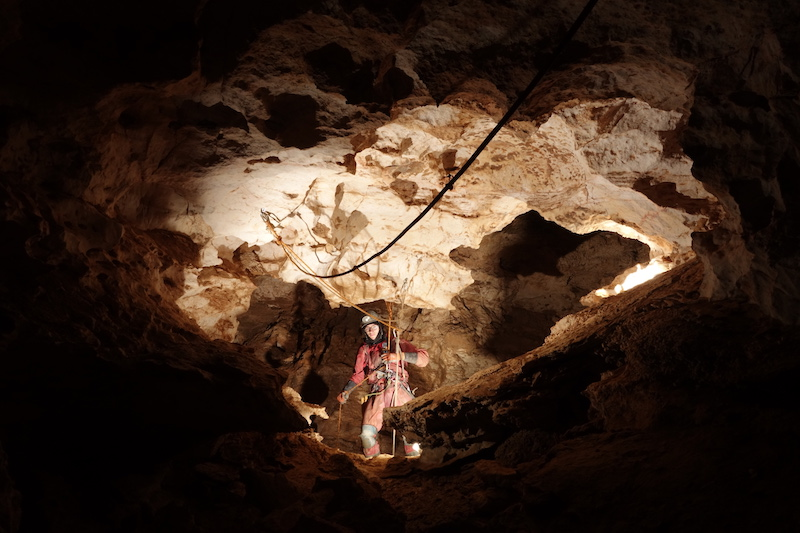
\includegraphics[width=\textwidth]{images/2016/arun-rescue-2016/knotverygood.jpg}}
        \caption{A caver negociating he top of Knot Very Good pitch, about 15 minutes away from Sejna Soba --- Rhys Tyers}
        \label{KnotVeryGood}
    \end{figure*}

    Tanguy, doing everything to keep me warm, removed my damp wetsocks and replaced them with his thick woollen socks. He and I then attempted to sleep, but I’m unsure if either of us slept more than a few minutes.
    Around 5am Clare returned. She had brought with her a stove and a few other bits. She and Tanguy helped me into a large, extremely well insulated ‘blizzard blanket’ which had chemical heat pads on the inside. I was fed codeine and noodles. Tanguy feeding me noodles with a spork inside a bothy bag was pretty amusing. The three of us rested inside the bothy bag for a while, and it was around 6am I believe when Tanguy left to exit the cave.

    Clare and I remained inside the bothy bag waiting for the Rescue to reach us. Again I don’t think either of us slept; Clare herself must have been extremely tired having not really rested. At one point she cooked smash with soup and chunks of cheese for the two of us, which I would rate a solid 9/10. My lack of appetite unfortunately limiting enjoyment.
    Fratnik and first medic arrived around 10:30am. She was very kind, asked me a few questions and tested my back, but it then took a while longer until the other medics followed behind, bringing with them a large medical kit. They cut the cuffs on my furry and oversuit to get a tourniquet on my forearm for a cannula to be placed in my right hand. As I was being treated as worst case I was given pain killers and steroids. When my temperature was taken it measured 37.6 degrees Celsius thanks to the effort of Will, Tanguy and Clare in keeping me warm in the 18 hours I was lying down.
    We had to wait then for the rest of the JRS to bring down the stretcher and prepare the cave for the rescue. Clare assisted in guiding the team through the cave, as most had not been in the system before.

    At around 12/1pm I was stretchered up first 2 pitches to Sane and Sober (can’t remember the Slovenian). I was stretchered horizontally for these first pitches, as they had easy enough pitch heads and there was no rush due to the preparations further up the system. For all the pitches after the first two I was pulled up vertically, I was comfortable enough like this and it made the rescue quicker and easier for the JRS. We had to pause for 1-2 hours at Sane and Sober as the Risanke squeezes required gardening and blasting to allow the JRS to pull me through on the stretcher. Whilst we waited they threw up a red bivvi, allowing some members of the team to rest. We weren’t given any immediate warning for the blasting so the explosions made us all jump a little, with smiles and chuckle all around.
    The effort the JRS put in to get me through Risanke was incredible. In a squeeze where there isn’t much room to manoeuvre they managed to hold up the stretcher and pull me through. When there was enough space, someone would be underneath the stretcher, helping shuffle me through. Every movement was careful and done together. When we had passed the toughest points everyone paused to rest and acknowledge the achievement. Truly an honour to experience.

    \begin{figure*}[t!]
        \checkoddpage \ifoddpage \forcerectofloat \else \forceversofloat \fi
        \centering
        \begin{subfigure}[t]{0.428\textwidth}
            \centering
            \frame{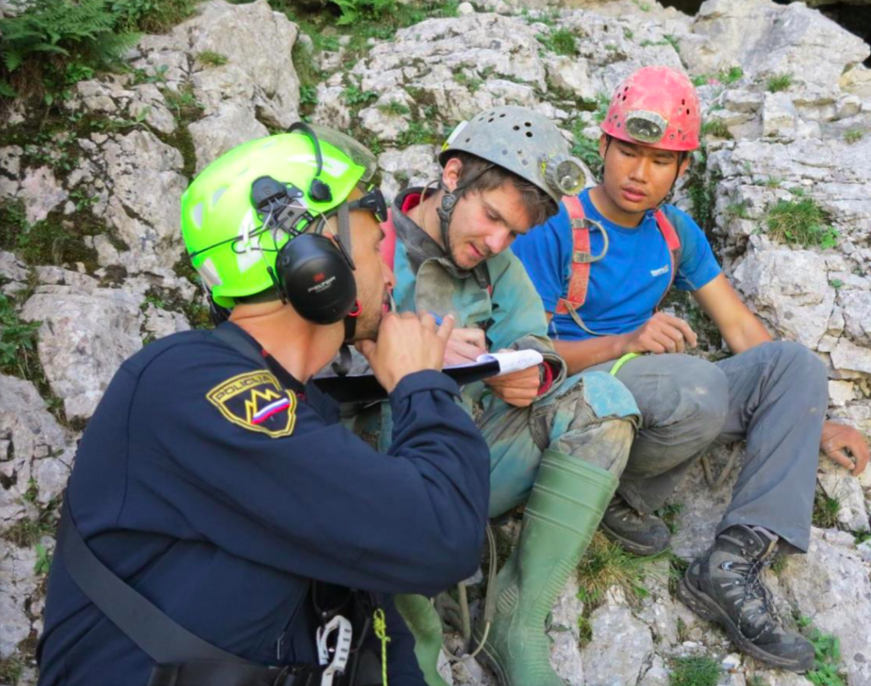
\includegraphics[width=\linewidth]{images/2016/arun-rescue-2016/passing_down_information}}
            \caption{}\label{information}
        \end{subfigure}
        \hfill
        \begin{subfigure}[t]{0.517\textwidth}
            \centering
            \frame{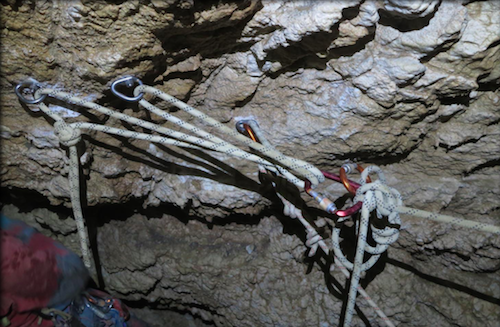
\includegraphics[width=\linewidth]{images/2016/arun-rescue-2016/preparing_stretcher}} 
            \caption{} \label{stretcher prepared}
        \end{subfigure}
            
         \vspace{0.3cm}

        \begin{subfigure}[t]{\textwidth}
            \centering
            \frame{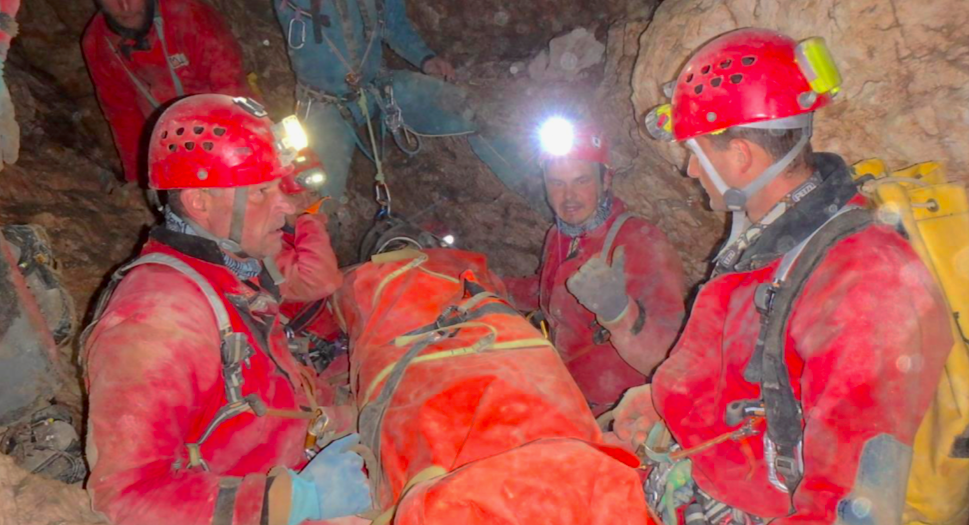
\includegraphics[width=\linewidth]{images/2016/arun-rescue-2016/moving_stretcher}} 
            \caption{} \label{stretcher moved}
        \end{subfigure}

            \caption{
            \emph{a} Will Scott and Kenneth Tan relaying information to the rescue team
            \emph{b} Newly placed tri-hangs allow the stretcher to be moved safely across the cave
            \emph{c} The rescue team with stretcher secured on cowstails move through horizontal sections of Primadona --- Maks Merela, deputy leader of the Slovenian Cave Rescue (JZS)}
    \end{figure*}


    I had on a helmet with a plastic guard to protect my face whilst my hands were strapped down, and with the action it had seen before, the scratches and scuffs had rendered it all but opaque. So it kept my mind active by trying to figure out where I was in the cave. With the different rigging set up by the JRS to accommodate the stretcher, my new perspective of the ceiling, the newly blasted passage and being a little drowsy from the painkillers and tiredness I was mostly lost. But I was kept informed of the immediate plans.

    The exit out of the cave after we had cleared Risanke followed a smooth system. Pause whilst the cave ahead was rigged to accommodate the stretcher, then an hour or so of activity where I was moved up through the cave. Occasionally a longer pause where the red bivvi would be strung up. I’m fairly sure I didn’t sleep during the rescue, I may have drifted off for a moments but was unable to switch off and get some rest.

    I don’t clearly recall the details of the last few hours of the rescue, I was very tired and finding it difficult to stay positive. Some of the rescuers including the medic who first came down with Fratnik were getting tired and cold as there were large breaks. As we reached the last few pitches near the entrance things began to drag out for me. They were really pushing to get me out of the cave in the window where the helicopter would be available, meaning at some pitches I was hanging in the stretcher for a while not moving whilst the immediate pitch was prepared. This was tiring but not painful, and necessary. The crawl at the bottom of the snowslope at the entrance was difficult for the team. It is at an angle where if they let go of the stretcher I would have slid down, and tight and low so difficult to support the stretcher. It was passed easily enough though, and not uncomfortably. Ascending up the snowslope was also tricky, the stretcher was on a rope but the rescuers either side of me were not. They dragged me up with care, despite it being difficult to maintain solid footholds and balance, and being at the end of a massive rescue effort.

    My exit out the cave is an image I cannot forget. We emerged at 2:11am on Sunday morning, 35 hours after I had been injured. My weariness disappeared instantly, replaced with my relief to be out as I took in the scene. The cliff was covered in 20-30 bright white headtorches, all pointed at us as I was now carried away from the entrance by the JRS and passed over to the mountain rescue. As I watched the faces of those carrying me, I looked past them at the Primadona entrance as there was a flash of lightning as a storm in the sky to the right moved in. I heard the whirr of a helicopter, and looking up away from the rescuers, I watched it drift across the storm, and then fly back across out of view, waiting for the call to pick me up. I was then attached to a rope line and lowered, slowly, past a flaming torch (a marker, for the helicopter) to a group of mountain rescuers on a small flat area of the mountain. They held me up as the helicopter came in towards us. I could feel the force of the air buffeting us and the overwhelming noise of the blades but I didn’t realise that the helicopter was hovering so close, at a level where I could be passed straight through the door and onto the cabin floor. The two pilots and the crew member were all wearing night vision goggles, and from my position on the floor I just lay still and became entranced by the noise and the pilots with their green dials for the 20/30 minute flight.

    When we landed at the hospital I experienced the contrast of the noise of the helicopter with the quiet of a hospital at 3am. I arrived and was quizzed, cut out of my oversuit, put on an IV drip and finally was able to take my contact lenses out. Having no identification I had to write out my personal information for the staff. I was wheeled out and x-rayed by staff who couldn’t talk to me in English. I was told that I had multiple fractures to my lower spine, but no indication that the spinal canal was compromised. I didn’t need any emergency surgery and was finally allowed to sleep at around 6am Sunday morning.

    My account of the rescue is a little blurry, I spent much of it half asleep and my vision was limited. I felt mostly terrified and entirely helpless from the time of my injury all the way up until I was being hauled up the first two pitches, when I very quickly realised the professional competency of the JRS. All members kept a calm and kind demeanour, in good spirits which was very comforting for me. There was quick, clear and constant communication between everyone and I was being checked on at every stage of the operation.

    \name{Arun Paul}
    \\
    \begin{figure*}
        \begin{tikzpicture}
            \node [name-dest] (box){%
                \begin{minipage}{\textwidth}
                    \begin{multicols}{2}
                        Only a couple of pitches inside the cave, and out into the calm, blue morning. By then the rescue had been called, it was being organised, but still in its infancy. The hardest shifts had been done, so I took my time on the last stretches of rope and staggered across the plateau to the bivi.

                        The Skalars, Janet, Will and Kenneth were up. I shared what news I had, had tea, ate vast quantities of bread, asked for the latest surface info. Kenneth and Will were going down to meet the first rescuers at the cave entrance with drill and rope. After meat and mead, I undressed by my tent and lay on the grass asking to be woken up after 8 hours so I could do more if needed. The sun saw to my waking up, after exactly an hour and a half. It became unbearably hot, so I retreated to the bivi. Upon Tetley’s advice I wrote down the series of events to the best of my knowledge then in the logbook.

                        The rest of the day was spent recuperating, visiting the snow chamber in M2 with the Skalars, Tetley, Dave, Will and Kenneth, and getting information from Karin via the walkie-talkies. In the late aftertoon Clare came back up, with more ample news, and tales of blasting and intense gardening that had held her up below Risanke for quite a time.

                        On Sunday, Tetley broke the news in the bivi, stating that Arun had been helicoptered back to Ljubljana. He himself had cooked with Zdenko in the Shepherd’s hut in Kal during the night, as rescuers streamed back from the cave entrance. With some four tacklesacks of gear left at the Cattlegrid pitch, Dave and I decided to descend down the cave to retrieve them. This was done smoothly, though we were rained on heavily during the final ascent.

                        \name{Tanguy Racine}
                  \end{multicols}
                \end{minipage}
            };
            \node[fancytitle, right=10pt] at (box.north west) {Epilogue};
        \end{tikzpicture}
    \end{figure*}


